% intro_v2.tex — Failure-Grounded Distillation framing
% Central question: distill vs. retrieve. Asymmetry finding moved up. No "first X" claims.
\section{Introduction}
\label{sec:introduction}



\begin{wrapfigure}{r}{0.5\linewidth}
\centering
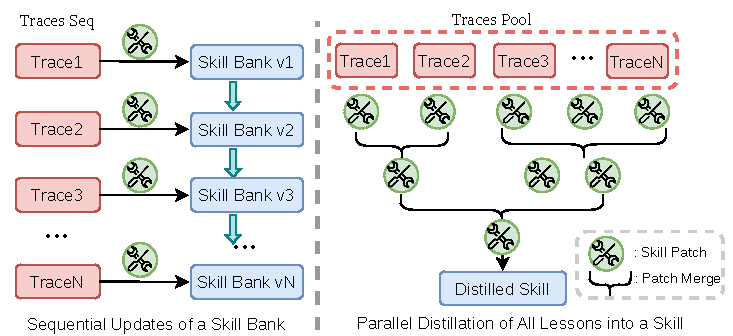
\includegraphics[width=\linewidth]{figures/intro_cropped.pdf}
\caption{\textbf{Left:} sequential online skill evolution edits the skill after each incoming trace. \textbf{Right:} \systemname{} analyzes many traces in parallel and hierarchically consolidates recurring lessons into one portable skill.}
\label{fig:intro}
\end{wrapfigure}


LLM-based agents increasingly rely on \emph{skills}: reusable documents that encode task procedures, domain knowledge, and operational guidelines \citep{anthropic2026skills,zhou2026comprehensivesurveyagentskills}.
As agents move into specialized file- and tool-use workflows, the bottleneck is no longer only model capability, but also the ability to create and maintain high-quality skills for each domain \citep{han2026sweskillsbenchagentskillsactually,li2026organizingorchestratingbenchmarkingagent,anthropic2026skillcreatorconversation,liang2026skillnetcreateevaluateconnect,zhou2026comprehensivesurveyagentskills}.
Human-written skills can help, but they are not uniformly beneficial across agents: in \cref{tab:main_v1}, the official \texttt{xlsx} skill improves a 122B spreadsheet agent while hurting a 35B agent on the same benchmark.
Generating skills purely from parametric knowledge is also brittle, because such drafts often lack the concrete failure modes, workarounds, and operational details exposed by actual execution traces \citep{li2026skillsbenchbenchmarkingagentskills,jiang2026xskillcontinuallearningexperience,zhou2026comprehensivesurveyagentskills}.

Recent systems therefore use agent experience to evolve skills or memories online \citep{yang2026autoskillexperiencedrivenlifelonglearning,xia2026skillrlevolvingagentsrecursive,alzubi2026evoskillautomatedskilldiscovery,zhou2026mementoskillsletagentsdesign,jiang2026xskillcontinuallearningexperience,zhou2026comprehensivesurveyagentskills}.
This direction is promising, but many existing approaches either store trajectory-local lessons for retrieval or edit skills sequentially as new traces arrive (\cref{fig:intro}, left).
Such designs can fragment reusable knowledge across a large memory or skill collection, and sequential editing can make later skills depend on the order of earlier updates \citep{li2026singleagentskillsreplacemultiagent}.
\textbf{Human experts usually work differently:} they inspect broad traces, abstract recurring patterns, and write compact procedures that are reusable across cases.

We introduce \systemname{}, a framework for turning execution traces into portable skills.
Rather than retrieving per-episode memories at test time or absorbing traces through order-dependent sequential edits, \systemname{} analyzes many traces jointly and consolidates recurring lessons into a single skill directory (\cref{fig:intro}, right).
The same mechanism supports two common use cases: \emph{deepening} an existing human-written skill and \emph{creating} a useful skill from a weak LLM-generated draft.
This many-to-one consolidation acts as an inductive reasoning step over agent experience \citep{xiong-etal-2025-co,li2025mirageevaluatingexplaininginductive,lin2025llmbasedscientificinductivereasoning}, while preserving the portability of ordinary skill files.

Experiments show that trajectory-grounded skills improve performance while remaining portable across models, benchmarks, and task domains.
In spreadsheet workflows, \systemname{} both strengthens Anthropic's official \texttt{xlsx} skill and creates useful skills from scratch.
The resulting skills transfer across model scales and families: for example, a skill evolved with Gemma-4-31B-it \citep{gemma42026} improves Qwen3.5-122B \citep{qwen35blog}.
They also generalize to out-of-distribution (OOD) data and tasks, such as transferring from spreadsheet editing to table QA.
The benefits extend beyond spreadsheets: \systemname{} improves math reasoning and DocVQA, and further strengthens Anthropic's official PDF, DOCX, and PPTX workflow skills.
Further analyses show that:
parallel consolidation is much faster and generally stronger than order-dependent skill editing; a single distilled skill outperforms ReasoningBank-style episodic retrieval \citep{ouyang2026reasoningbankscalingagentselfevolving}; and agentic analysts produce better patches by inspecting artifacts and validating fixes.
Qualitatively, the learned patches are not trajectory-specific tips: they coalesce into reusable SoPs, while patch-selection studies show that their value is often combinatorial, making holistic consolidation more reliable than greedy local selection. 

We contribute: (1) \textbf{Trace2Skill}, a framework for automatic skill creation and deepening. It mirrors human skill writing: building broad prior knowledge through extensive trajectory analysis before drafting skills (\cref{sec:method}). (2) \textbf{Broad empirical evidence} that trajectory-grounded evolution yields skills that transfer effectively across LLM scales, families, and OOD tasks (\cref{sec:experiments}). (3) \textbf{Comprehensive analysis} showing why consolidation works: parallel merging improves over sequential updates, one consolidated skill beats retrieval-based reasoning memories, agentic diagnosis improves patch quality, and patch value is often combinatorial (\cref{sec:analysis}).

\begin{figure}[t]
    \centering
    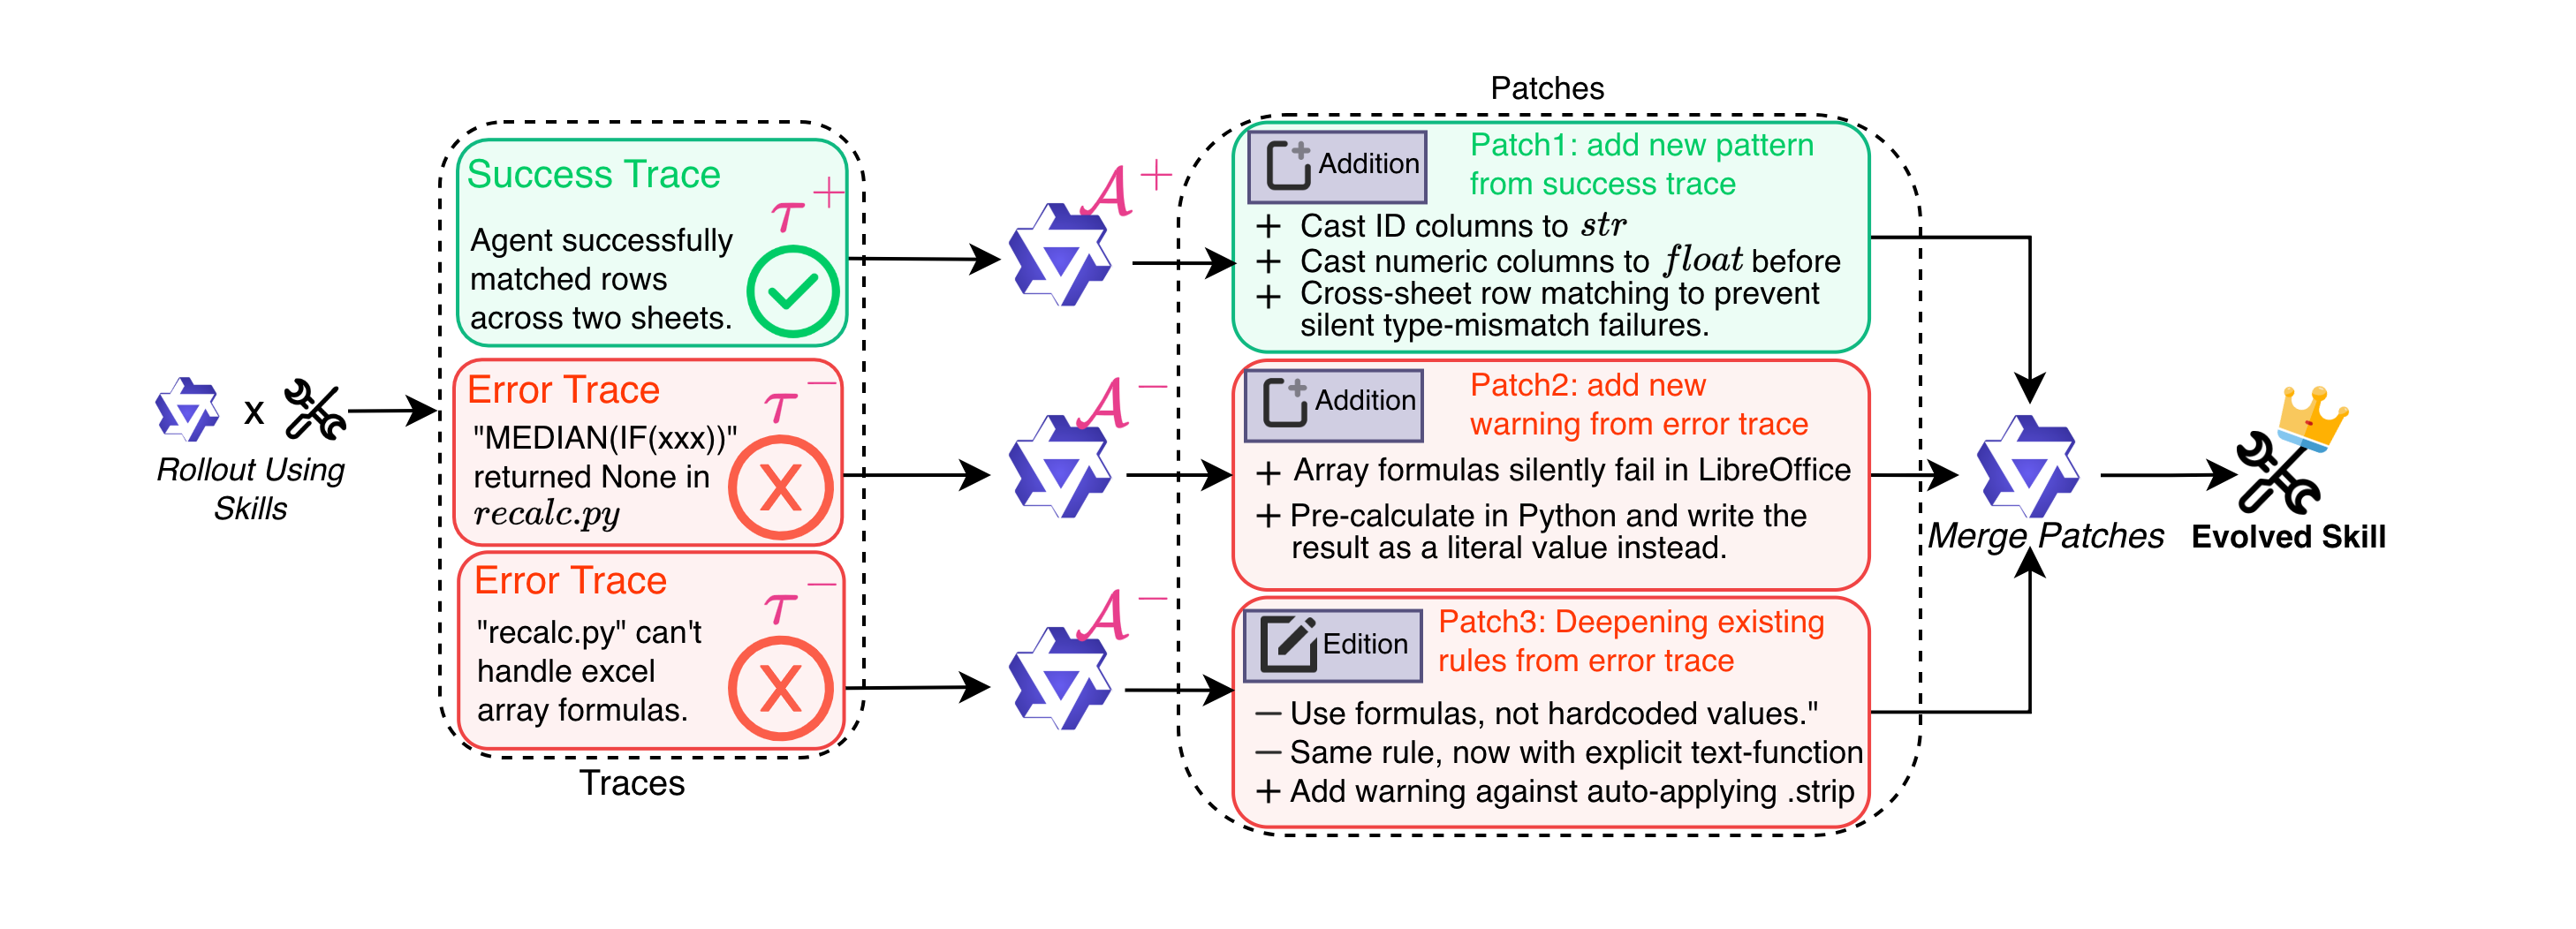
\includegraphics[width=\linewidth]{figures/trace2skill_framwork}
    \caption{Overview of \systemname{}'s three-stage pipeline: (1)~roll out a frozen agent to collect labeled success and failure trajectories, (2)~propose trajectory-level skill patches in parallel with separate error and success analysts, and (3)~hierarchically merge all patches into one portable skill directory.}
    \label{fig:pipeline}
\end{figure}

% \begin{itemize}[leftmargin=*]
%     \item \textbf{Trace2Skill}, a framework for automatic skill creation and deepening. It mirrors human skill writing: building broad prior knowledge through extensive trajectory analysis before drafting skills (\cref{sec:method}).

%     \item \textbf{Broad empirical evidence} that trajectory-grounded evolution yields skills that transfer effectively across LLM scales, families, and out-of-distribution tasks (\cref{sec:experiments}).

%     \item \textbf{Comprehensive analysis} showing why consolidation works: parallel merging improves over sequential updates, one consolidated skill beats retrieval-based reasoning memories, agentic diagnosis improves patch quality, and patch value is often combinatorial (\cref{sec:analysis}).
% \end{itemize}
